\documentclass[12pt,a4paper]{article}
\usepackage[english]{babel}
\usepackage[utf8x]{inputenc}
\usepackage[T1]{fontenc}
\usepackage{listings}
\usepackage{amsfonts}
\usepackage{amssymb}
\usepackage{amsmath,amsthm}
\usepackage{mathtools}
\usepackage{graphicx}
\newcommand{\comp}{\overline{\phantom{A}}}
\setlength{\tabcolsep}{12pt}

\newtheorem{theorem}{Theorem}[section]
\newtheorem{lemma}[theorem]{Lemma}
\newtheorem{claim}[theorem]{Claim}
\newtheorem{proposition}[theorem]{Proposition}
\newtheorem{corollary}[theorem]{Corollary}
\newtheorem{fact}[theorem]{Fact}
\newtheorem{example}[theorem]{Example}
\newtheorem{notation}[theorem]{Notation}
\newtheorem{observation}[theorem]{Observation}
\newtheorem{conjecture}[theorem]{Conjecture}
\newtheorem{remark}[theorem]{Remark}
\newtheorem{definition}[theorem]{Definition}

\voffset=-0.6truein		% LaTeX has too much space at page top
\addtolength{\textheight}{0.3truein}
\addtolength{\textheight}{\topmargin}
\addtolength{\topmargin}{-\topmargin}
\textwidth  6.0in		% LaTeX article default 360pt=4.98''
\oddsidemargin 0pt	% \oddsidemargin  .35in   % default is 21.0 pt
\evensidemargin 0pt	% \evensidemargin .35in   % default is 59.0 pt

\title{Cylindric Set Algebras as an Extensions of Boolean Algebras}

\begin{document}
	%\MakeScribeTop
	

	
\maketitle

I will define cylindric set algebras and give two interpretations of a cylindric set algebra, geometric and logical. Then I will go over cylindrifications, diagonalizations and some basic results to give an introduction to cylindric algebras.

\section{Cylindric Algebra}

\begin{definition}
A \textbf{cylindric algebra} of dimension $\alpha$, for some ordinal $\alpha$, is an algebraic structure 
\begin{align*}
    \mathfrak{A} = \left< A,+,\cdot,-,0,1,\mathbf{c}_\kappa,\mathbf{d}_{\kappa\lambda}\right>_{\kappa,\lambda<\alpha}
\end{align*}
such that $0,1$ and \textbf{d$_{\kappa\lambda}$} are distinguished elements of $A$, \textbf{c$_\kappa$} are unary operations on $A$, $+$ and $\cdot$ are binary operations on $A$ satisfying\\\newline
\begin{tabular}{l}
    \textbf{C}$_0$ $\left<A,+,\cdot,-,0,1\right>$  is a Boolean algebra\\
    \textbf{C}$_1$ $\mathbf{c_\kappa}0 = 0$ \\
    \textbf{C$_2$} $x\le \mathbf{c_\kappa}x \;\;(x+\mathbf{c_\kappa}x=\mathbf{c_\kappa}x$)\\
    \textbf{C$_3$} $\mathbf{c_\kappa}(x\cdot\mathbf{c_\kappa}y)=\mathbf{c_\kappa}x\cdot\mathbf{c_\kappa}y$\\
    \textbf{C$_4$} $\mathbf{c_\kappa}\mathbf{c_\lambda}x=\mathbf{c_\lambda c_\kappa}x$\\
    \textbf{C$_5$} $\mathbf{d_{\kappa\kappa}}=1$\\
    \textbf{C$_6$} if $\kappa\neq\lambda,\mu$, then $\mathbf{d_{\lambda\mu}}=\mathbf{c_\kappa(d_{\lambda\kappa}\cdot d_{\kappa\mu})}$\\
    \textbf{C$_7$} if $\kappa\neq \lambda$, then $\mathbf{c_\kappa(d_{\kappa\lambda}\cdot x)\cdot c_\kappa(d_{\kappa\lambda}\cdot -x)}=0$
\end{tabular}
\end{definition}

The elements $\mathbf{d_{\kappa\lambda}}$ are called the diagonal elements and the operations $\mathbf{c_\kappa}$ are called cylindrifications. A cylindric algebra may not contain the diagonal elements, $\mathbf{d_{\kappa\lambda}}$, it will then be considered diagonal free. There are couple ways to think of these elements, geometrically drawing cylinders and also in the context of first-order logic. 

\section{Geometry}

\begin{definition}
($i$) For any set $U$, any ordinal $\alpha$, and any $\kappa<\alpha$ we let $\mathbf{C_\kappa}$ be the function $\mathcal{P}(\prescript{\alpha}{}{U})\to\mathcal{P}(\prescript{\alpha}{}{U})$ such that 
\begin{align*}
    \mathbf{C_\kappa}X =\{y:y\in \prescript{\alpha}{}{U} \text{\; and for some \;} x\in X\text{\; we have  \;} y_\lambda = x_\lambda \; \forall \lambda\neq\kappa\}
\end{align*}
for every $X\subseteq \prescript{\alpha}{}{U}$.\newline
($ii$) For any set $U$, any ordinal $\alpha$, and any $\kappa,\lambda<\alpha$, $\mathbf{D_{\kappa\lambda}}=\{y:y\in\prescript{\alpha}{}{U},y_\kappa=y_\lambda\}$\newline
($iii$) A is an $\alpha$\textbf{-dimensional cylindric field of sets} if there is a set $U$, called the \textbf{base} of $A$, such that $A$ is a non-empty subset of $\mathcal{P}(\prescript{\alpha}{}{U})$ closed under the operations $\bigcap,\bigcup,{}^c$ and $\mathbf{C_\kappa}$ for $\kappa<\alpha$ and containing all the sets $\mathbf{D_{\kappa\lambda}}$ \newline
($iv$) $\mathfrak{A}$ is a \textbf{cylindric set algebra of dimension} $\alpha$ \textbf{with base } $U$ if $\mathfrak{A}=\left<A,\bigcup,\bigcap,{}^c,0,\prescript{\alpha}{}{U},\mathbf{C_\kappa},\mathbf{D_{\kappa\lambda}}\right>_{\kappa,\lambda<\alpha}$ where $A$ is an $\alpha$-dimensional cylindric field of sets with base $U$
\end{definition}

The set $\prescript{\alpha}{}{U}$ is the $\alpha^\text{th}$ cartesian product of $U$, ie. the set with $\alpha$ tuples of elements from $U$. A set $X$ such that $X=\mathbf{C_\kappa}X$ is called a cylinder parallel to the $\kappa^\text{th}$ axis, or a $\kappa$-cylinder.
\newline

As an example, consider $\prescript{2}{}{U}$. We see in the figures below the cylindrifications of some sets $X,Y\subset \prescript{2}{}{U}$ and verify the axiom \textbf{C$_3$}.

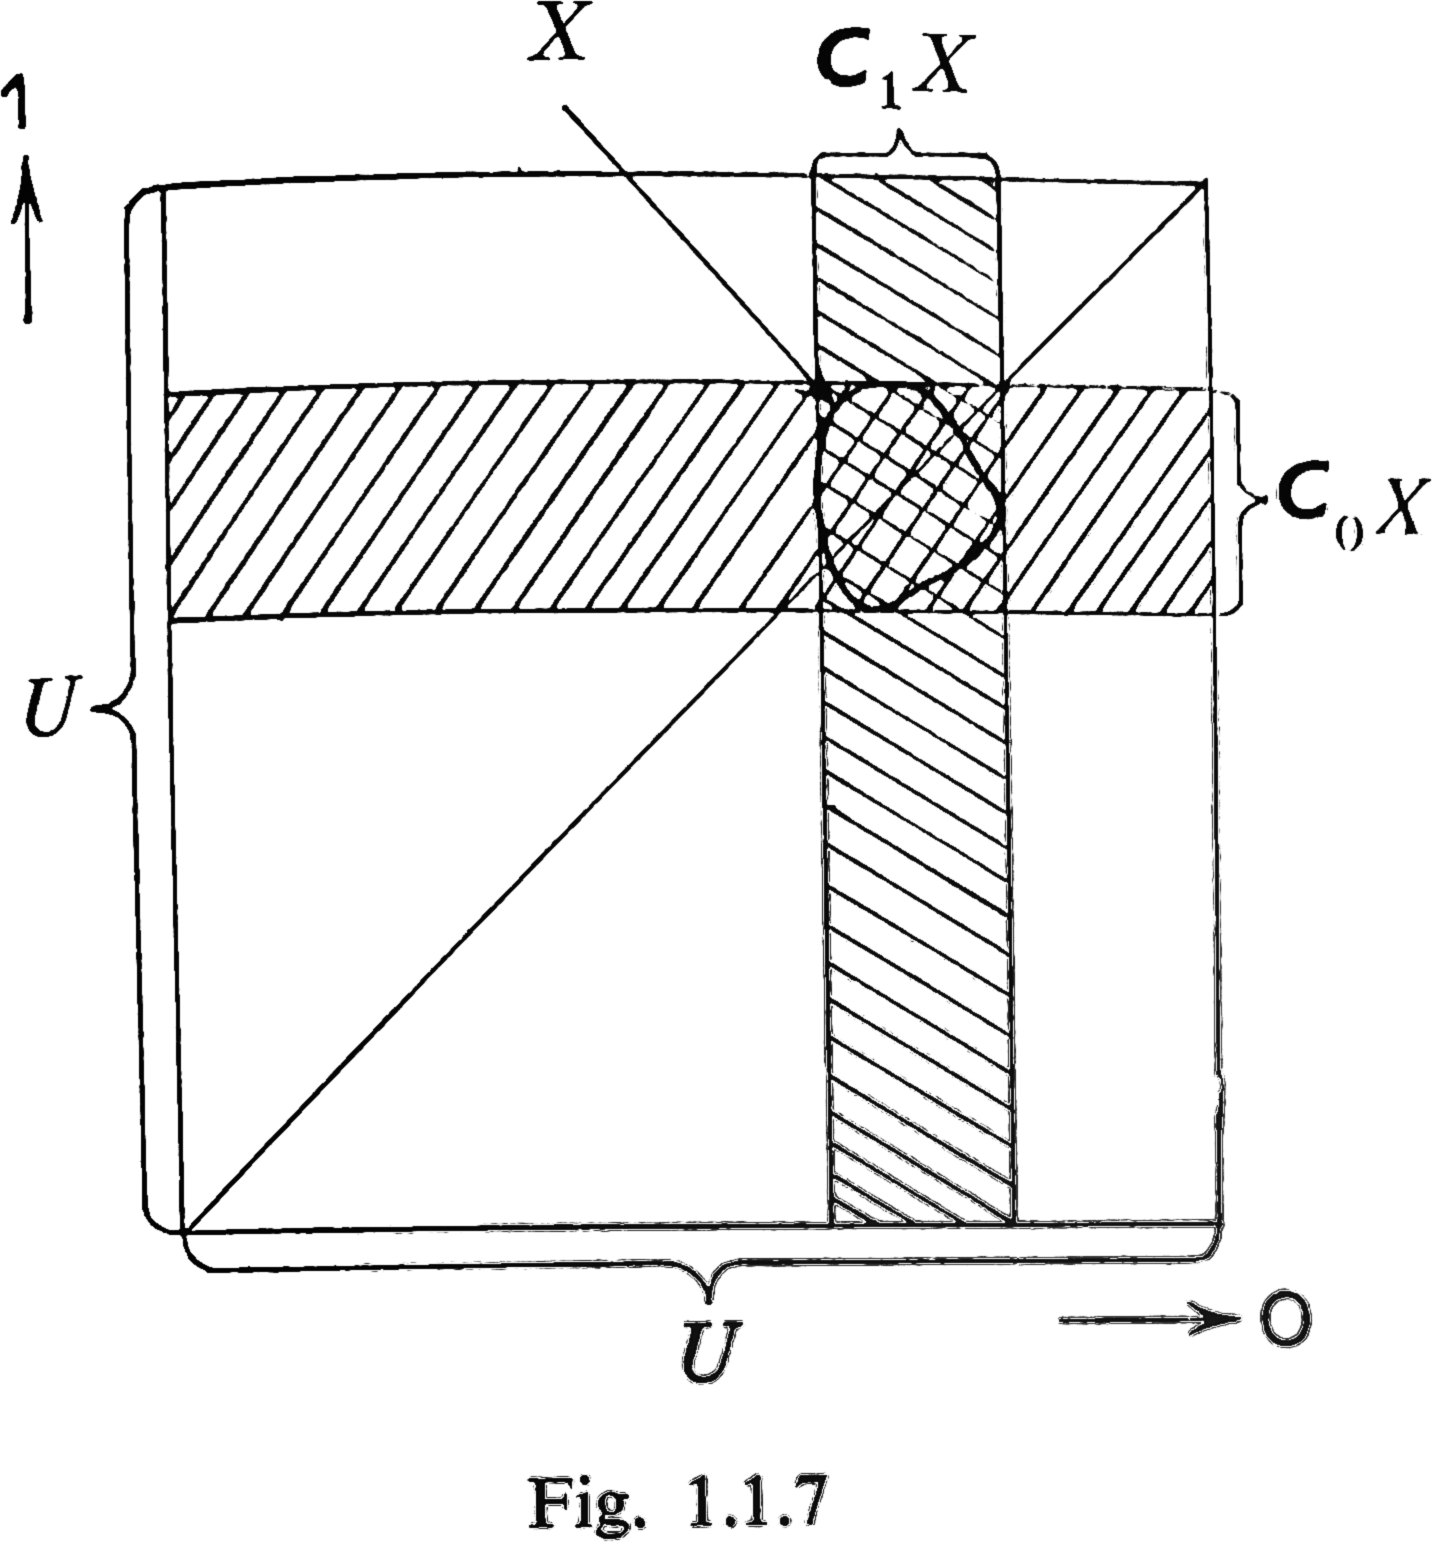
\includegraphics[scale=0.1]{Cylindrification1.png}
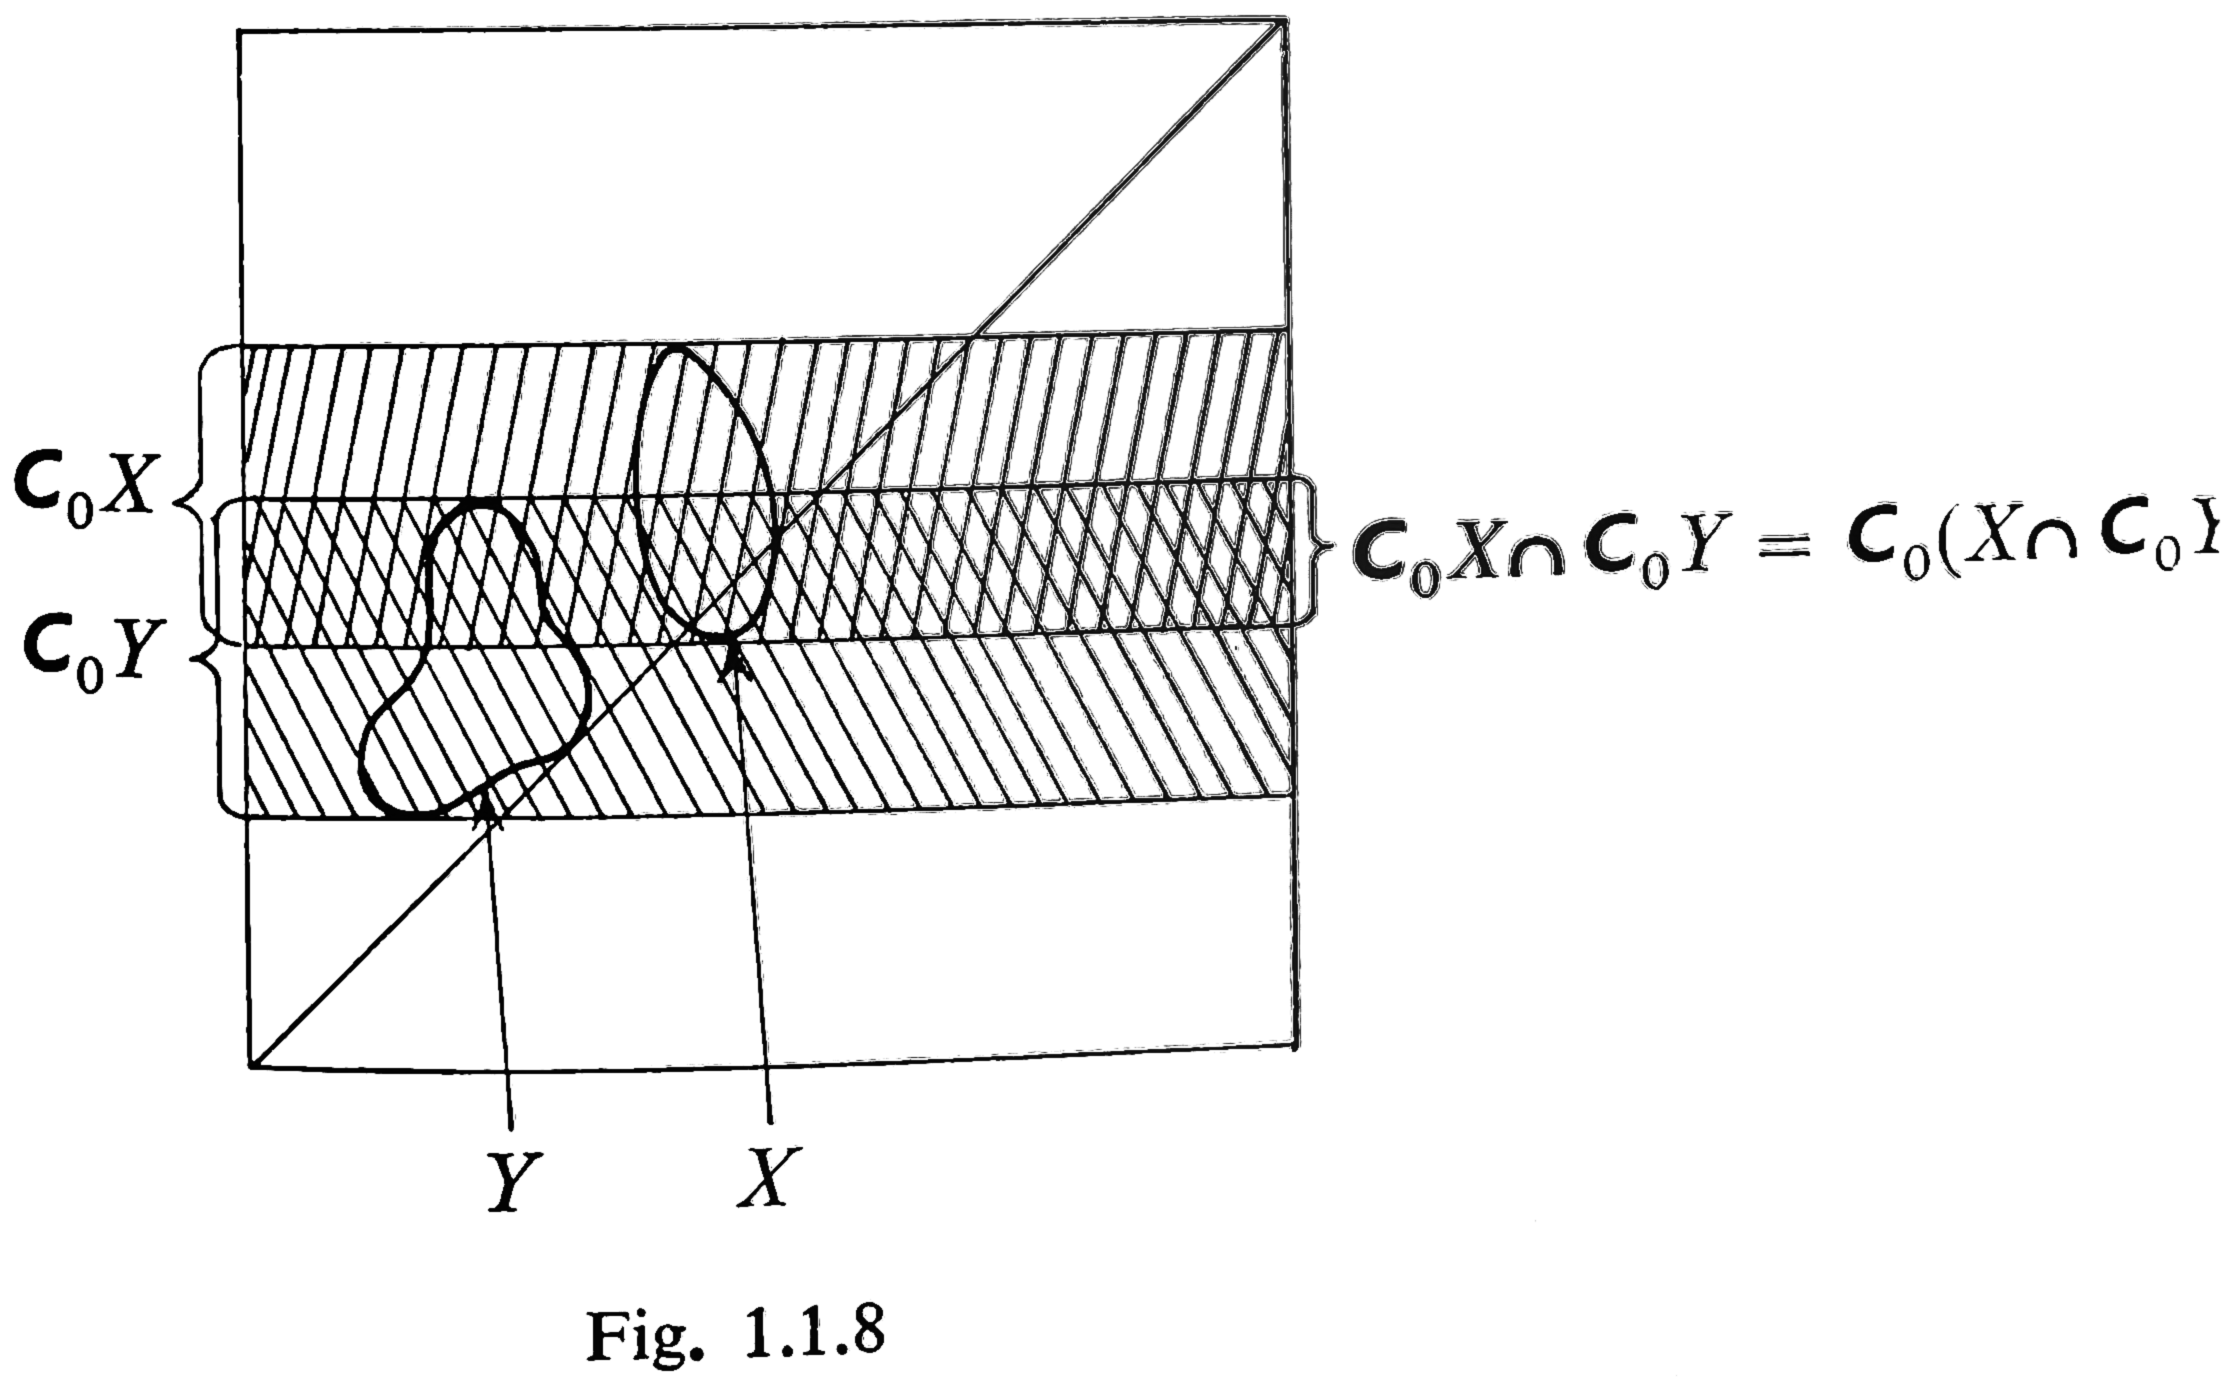
\includegraphics[scale=0.1]{Cylindrification2.png} 


\section{First-order Logic}


\begin{definition}
For a language $\Lambda$ of predicate logic we let $\mathfrak{Fm}^{(\Lambda)}$ be the algebra 
\begin{align*}
    \left< \Phi\mu^{(\Lambda)},\vee,\wedge,\neg,\bot,\top,\exists_{v_\kappa},v_\kappa=v_\lambda\right>_{\kappa,\lambda<\alpha}
\end{align*}
where $\alpha$ is the length of the sequence of variables of $\Lambda$. $\mathfrak{Fm^{(\Lambda)}}$ is called the free algebra of formulas in $\Lambda$.
\end{definition}

\begin{theorem}
If $\Sigma$ is a set of sentences of $\Lambda$, then $\equiv_\Sigma$ is a congrunece relation on $\mathfrak{Fm}^{(\Lambda)}$ where $\sigma\equiv_\Sigma\tau \iff\Sigma \vdash \sigma=\tau$ and $\mathfrak{Fm}^{(\Lambda)}/\equiv_\Sigma$ is a cylindric algebra, similar to the construction of the Lindenbaum-Tarski Boolean algebra.
\end{theorem}

The algebra $\mathfrak{Fm}^{(\Lambda)}/\equiv_\Sigma$ is called the cylindric algebra of formulas in $\Lambda$ with respect to $\Sigma$. As well, we can restrict our notion to only theories, instead of sets of sentences, without loss of generality.

\section{Cylindrifications}

As an example for the use of cylindric algebras, consider the following theorem: $\phi \wedge \exists x(\psi) = \bot \iff \psi\wedge\exists y(\phi)$. This can be reworded in the terms of cylindric algebras in the following theorem.

\begin{theorem}
$x \cdot \mathbf{c_\kappa}y=0\iff y\cdot \mathbf{c_\kappa} x=0$
\end{theorem}
\begin{proof}
By \textbf{C}$_3$ we have $\mathbf{c_\kappa}(x\cdot\mathbf{c_\kappa}y)=\mathbf{c_\kappa}(y\cdot\mathbf{c_\kappa}x)$, then the proof is complete by noticing $\mathbf{c_\kappa}x=0\iff x=0$.
\end{proof}

Some results about the lattice structure:

\begin{theorem}
$\mathbf{c_\kappa}(x+y)=\mathbf{c_\kappa}x+\mathbf{c_\kappa}y$
\end{theorem}

\begin{corollary}
$x\le y \iff \mathbf{c_\kappa}x\le\mathbf{c_\kappa}y$, in particular, $x\le\mathbf{c_\kappa}y\iff\mathbf{c_\kappa}x\le\mathbf{c_\kappa}y$
\end{corollary}

\begin{theorem}
$\mathbf{c_\kappa}x\cdot\mathbf{c_\lambda}y=0\iff\mathbf{c_\lambda}x\cdot\mathbf{c_\kappa}y=0$
\end{theorem}

And now, the cylindrification of a Boolean algebra is done as follows:

\begin{theorem}
If $\left<A,+,\cdot,-,0,1\right>$ is a Boolean algebra and $f$ a function on $A$ defined as
\begin{align*}f=\begin{cases}
0 & x=0\\
1 & x\neq 0
\end{cases}\end{align*}
Then $\left<A,+,\cdot,-,0,1,f,1\right>$ is a cylindric algebra and $\left<A,+,\cdot,-,0,1,f\right>$ is a diagonal free cylindric algebra
\end{theorem}

\section{Diagonal Elements}

\begin{definition}
$\mathfrak{A}$ is called \textbf{discrete} if $\mathbf{d_{\kappa\lambda}}=1$ and $\mathbf{c_\kappa}x=x$ for all $\kappa,\lambda<\alpha$ and all $x\in A$.
\end{definition}
Discrete cylindric algebras are degenerate and typically ruled out of consideration.
In particular, a cylindric algebra of formulas associated with a theory is discrete if and only if $\forall x\forall y (x=y)$ is valid in the theory.

\begin{theorem}
For any $\kappa$, the following are equivalent:
\begin{align*}
    (i)& \mathfrak{A} \text{  is a discrete cylindric algebra of dimension  }\alpha\\
    (ii)& \forall x, \mathbf{c_\kappa}x=x\\
    (iii)& \forall \lambda\neq \kappa, \mathbf{d_{\kappa\lambda}}=1
\end{align*}
\end{theorem}

\begin{corollary}
If $\mathfrak{A}$ is not discrete, then $|\alpha|\le |A|$. In particular, every non-discrete cylindric algebra of dimension $\alpha\ge \omega$ must be infinite
\end{corollary}

\section{Atoms}
\begin{definition}
The \textbf{dimension set} of $x$, $\Delta x$, is the set of all $\kappa$ such that $\mathbf{c_\kappa}x\neq x$
\end{definition}

In our geometric notion of clyindric set algebras, $\Delta X$ is the set of $\kappa<\alpha$ such that $X$ does not form a cylinder parallel to the $\kappa^{th}$ axis.
In terms of cylindric algebra of formulas associated with a theory $\Phi$, $\Delta(\phi/\equiv_\Phi)$ consists of all $\kappa<\alpha$ such that $\exists_{v_\kappa}\phi\iff\phi$, hence contains only those $\kappa$ for which $v_\kappa$ is free in $
\phi$.

\begin{theorem}
$\Delta 0=\Delta 1=\emptyset$, $\mathfrak{A}$ is discrete if and only if $\Delta x=0$ and for all $x\in A$
\end{theorem}

\begin{definition}
Let $\Gamma$ be a subset of $\alpha$, $x$ is called a $\mathbf{(\Gamma)}$\textbf{-closed} element or a $\mathbf{(\Gamma)}$\textbf{-cylinder} if $\Delta x\bigcap \Gamma=0$. The set of $\Gamma$-closed elements is denoted $\text{Cl}_\Gamma\mathfrak{A}$ and let $\mathfrak{Cl}_\Gamma\mathfrak{A}=\left<\text{Cl}_\Gamma\mathfrak{A},+,\cdot,-,0,1\right>$.
\end{definition}

\begin{theorem}
$\mathfrak{Cl}_\Gamma\mathfrak{A}$ is a Boolean algebra for every $\Gamma\subseteq\alpha$
\end{theorem}

The atoms of a cylindric algebra $\mathfrak{A}$ are the atoms of the Boolean part, denoted \textit{At}$\mathfrak{A}$.
\begin{definition}
A $\Gamma$\textbf{-atom} of $\mathfrak{A}$ is an atom of $\mathfrak{Cl}_\Gamma\mathfrak{A}$, ie. an element of \textit{At}$\mathfrak{Cl}_\Gamma\mathfrak{A}$.
\end{definition}

Geometrically, the singleton atoms are the $\{\kappa\}$-atoms which are lines parallel to the $\kappa$-axis.
$\Gamma$-atoms are linear subspaces parallel to the subspace spanned by the set of all $\lambda$-axes for $\lambda\in\Gamma$.

\begin{corollary}
In particular, the $0$-atoms of $\mathfrak{A}$ correspond with the atoms of $\mathfrak{A}$, At$\mathfrak{Cl}_0\mathfrak{A}=\mathit{At}\mathfrak{A}$
\end{corollary}

A particular type of atom that is interesting are rectangular elements.

\begin{definition}
$\mathbf{c_{(0)}}x=x$ and, if $\Gamma$ is a non-empty finite subset of $\alpha$, $\mathbf{c_{(\Gamma)}}x=\mathbf{c_{\kappa_0}\cdot\ldots\cdot c_{\kappa_{\lambda-1}}x}$ for all $x\in A$ where $|\Gamma|=\lambda$ and $\left<\kappa_0,\ldots,\kappa_{\lambda-1}\right>$ is the strictly increasing sequence whose range is $\Gamma$.
\end{definition}

\begin{definition}
An element $x$ is \textbf{rectangular} if $\mathbf{c_{(\Gamma)}}x\cdot\mathbf{c_{(\Delta)}}x=\mathbf{c_{(\Gamma\bigcap\Delta)}}x$ for all $\Gamma$ and $\Delta$. 
\end{definition}

The rectangular elements of a $2$-dimensional cylindric set algebra are exactly the elements that can be drawn as rectangles.
In an arbitrary finite dimension $\alpha$, the rectangular sets, X, are "generalized boxes", those sets which are Cartesian products of their projections on all coordinate axes
\begin{align*}
    X=\prod\limits_{\kappa<\alpha} \pi_\kappa\left( X\right)
\end{align*}

\end{document}